\documentclass[12pt]{article}

\usepackage{amsmath}
\usepackage{unicode-math}
\usepackage{xltxtra}
\usepackage{xgreek}

\setmainfont{Liberation Serif}

\usepackage{tabularx}

\pagestyle{empty}

\usepackage{geometry}σ
 \geometry{a4paper, total={190mm,275mm}, left=10mm, top=10mm}

 \usepackage{graphicx}
 \graphicspath{ {images/} }

 \usepackage{wrapfig}
\usepackage{lipsum}%% a garbage package you don't need except to create examples.

\begin{document}

\begin{table}
    \small
    \begin{tabularx}{\textwidth}{ c X r }
        \begin{tabular}{ c }
            
\includegraphics[scale=0.4]{logo}              \\
            ΕΛΛΗΝΙΚΗ ΔΗΜΟΚΡΑΤΙΑ                            \\
            ΥΠΟΥΡΓΕΙΟ ΠΑΙΔΕΙΑΣ, ΕΡΕΥΝΑΣ \& ΘΡΗΣΚΕΥΜΑΤΩΝ    \\
            ΠΕΡΙΦΕΡΕΙΑΚΗ Δ/ΝΣΗ ΠΡΩΤ. \& ΔΕΥΤ/ΜΙΑΣ  ΕΚΠ/ΣΗΣ \\
            ΚΕΝΤΡΙΚΗΣ ΜΑΚΕΔΟΝΙΑΣ                           \\
            Δ/ΝΣΗ ΔΕΥΤΕΡΟΒΑΘΜΙΑΣ ΕΚΠ/ΣΗΣ ΑΝ. ΘΕΣ/ΝΙΚΗΣ     \\
            27ο ΓΕΝΙΚΟ ΛΥΚΕΙΟ ΘΕΣ/ΝΙΚΗΣ
        \end{tabular}
         &  &
        \begin{tabular}{ r }
            Σχολικό Έτος: 2016 - 2017           \\
            Εξ. Περίοδος: Μαΐου - Ιουνίου       \\
            Μάθημα: Γεωμετρία Β Λυκείου         \\
            Εισηγητές: Λόλας, Φρύδας, Τερζόγλου \\ \\
            Θεσσαλονίκη, 24 / 05 / 2017
        \end{tabular}
    \end{tabularx}
\end{table}

\part*{\centering{Θέματα}}
\section*{Θέμα Α}
\noindent
\begin{enumerate}
    \item \textbf{[Μονάδες 15]} Να αποδείξετε ότι σε κάθε ορθογώνιο τρίγωνο, το τετράγωνο του ύψους που αντιστοιχεί στην υποτείνουσα ισούται με το γινόμενο των προβολών των κάθετων πλευρών στην υποτείνουσα
    \item \textbf{[Μονάδες 10]}  Να χαρακτηρίσετε τις παρακάτω προτάσεις με Σωστό ή Λάθος
          \begin{enumerate}
              \item [α)] Το τετράγωνο της κάθετης πλευράς ενός ορθογωνίου τριγώνου ισούται με το γινόμενο της κάθετης πλευράς με την υποτείνουσα.
              \item [β)] Το μήκος ενός τόξου $α$ ακτινίων σε κύκλο ακτίνας $R$ είναι $l=αR$.
              \item [γ)] Ο λόγος ομοιότητας των εμβαδών δύο όμοιων σχημάτων ισούται με τον λόγο ομοιότητας των πλευρών του.
              \item [δ)] Κανονικό πολύγωνο είναι αυτό που έχει όλες τις πλευρές του ίσες.
              \item [ε)] Σε τρίγωνο με πλευρές $α$, $β$, $γ$, αν ισχύει $β^2<α^2+γ^2$ τότε $\hat{Β}<90^{\circ}$.
          \end{enumerate}
\end{enumerate}

\section*{Θέμα Β}
\noindent
\begin{wrapfigure}[2]{r}{0.4\textwidth}
    \centering
    \vspace{-20pt}
    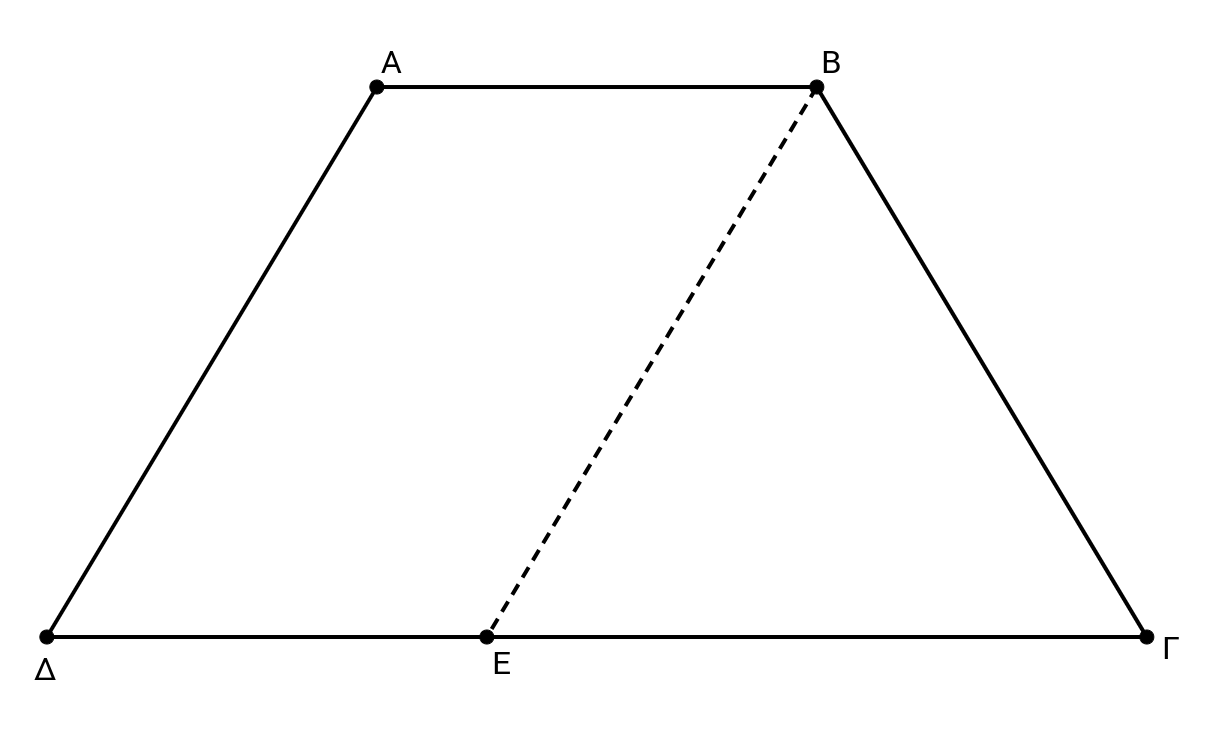
\includegraphics[width=0.4\textwidth]{2017BGeo2}
\end{wrapfigure}
Δίνεται ισοσκελές τραπέζιο $ΑΒΓΔ$ με $ΑΔ=ΒΓ=5$, $ΑΒ=4$ και $ΓΔ=10$. Από το $Β$ φέρνουμε παράλληλη προς την $ΑΔ$ που τέμνει την $ΓΔ$ στο $Ε$.
\begin{enumerate}
    \item \textbf{[Μονάδες 5]}  Να βρείτε το ύψος του τραπεζίου.
    \item \textbf{[Μονάδες 5]}  Να δείξετε ότι $(ΑΒΕΔ)=16$.
    \item \textbf{[Μονάδες 5]}  Να βρείτε το εμβαδό του τραπεζίου.
    \item \textbf{[Μονάδες 5]}  Να υπολογίσετε την ακτίνα του περιγεγραμμένου κύκλου στο τρίγωνο $\overset{\triangle}{ΒΓΕ}$
    \item \textbf{[Μονάδες 5]}  Να υπολογίσετε την ακτίνα του εγγεγραμμένου κύκλου στο τρίγωνο $\overset{\triangle}{ΒΓΕ}$
\end{enumerate}

\section*{Θέμα Γ}
\noindent
\begin{wrapfigure}[3]{r}{0.38\textwidth}
    \centering
    \vspace{-50pt}
    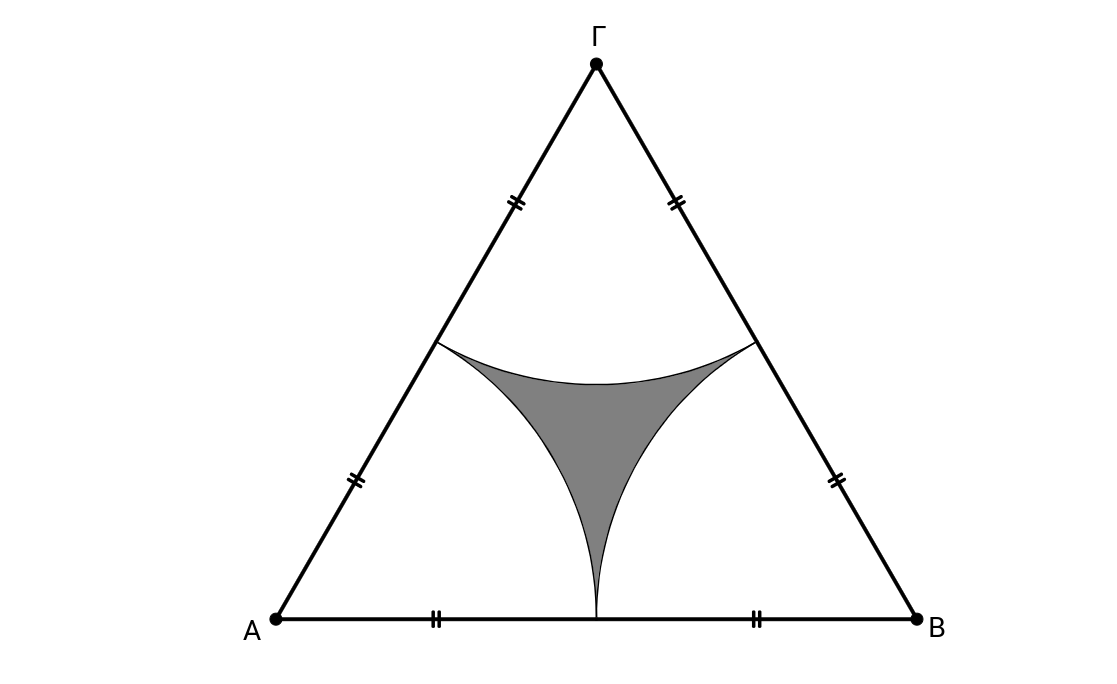
\includegraphics[width=0.38\textwidth]{2017BGeo3}
\end{wrapfigure}

Έστω ισόπλευρο τρίγωνο πλευράς $2R$. Με κέντρο κάθε κορυφή εγγράφουμε στο τρίγωνο κυκλικούς τομείς ακτίνας $R$ όπως το διπλανό σχήμα.
\begin{enumerate}
    \item \textbf{[Μονάδες 9]}  Να βρείτε την περίμετρο του γραμμοσκιασμένου σχήματος.
    \item \textbf{[Μονάδες 4]}  Να δείξετε ότι το ύψος του τριγώνου είναι $R\sqrt{3}$.
    \item \textbf{[Μονάδες 3]}  Να δείξετε ότι το εμβαδό του τριγώνου είναι $R^2\sqrt{3}$.
    \item \textbf{[Μονάδες 9]}  Να υπολογίσετε το εμβαδό του γραμμοσκιασμένου τμήματος.
\end{enumerate}

\section*{Θέμα Δ}
\noindent
\begin{wrapfigure}[1]{r}{0.4\textwidth}
    \centering
    \vspace{-50pt}
    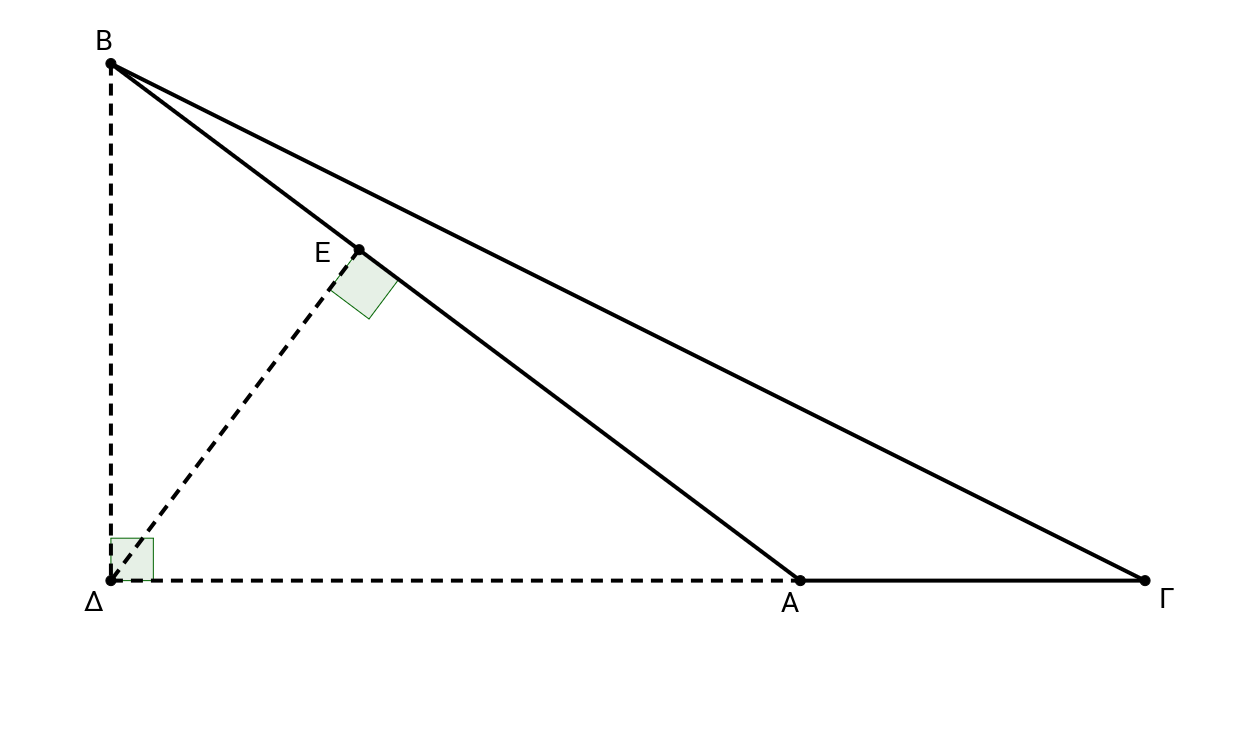
\includegraphics[width=0.4\textwidth]{2017BGeo4}
\end{wrapfigure}

Έστω τρίγωνο $\overset{\triangle}{ΑΒΓ}$ με $ΑΒ=25$, $ΒΓ=15\sqrt{5}$ και $συν\hat{Β}=\frac{11}{5\sqrt{5}}$.

\begin{enumerate}
    \item \textbf{[Μονάδες 5]}  Να δείξετε ότι $ΑΓ=10$.
    \item \textbf{[Μονάδες 5]}  Να αποδείξετε ότι το τρίγωνο $\overset{\triangle}{ΑΒΓ}$ είναι αμβλυγώνιο.
    \item \textbf{[Μονάδες 5]}  Να αποδείξετε ότι η προβολή $ΑΔ$ της πλευράς $ΑΒ$ στην πλευρά $ΑΓ$ είναι ίση με $20$.
\end{enumerate}

Στο τρίγωνο $\overset{\triangle}{ΔΒΑ}$ φέρνουμε το ύψος $ΔΕ \bot ΑΒ$. Να υπολογίσετε:
\begin{enumerate}
    \item [4.] \textbf{[Μονάδες 5]}  Την προβολή της $ΑΔ$ στην $ΑΒ$.
    \item [5.] \textbf{[Μονάδες 5]}  Το ύψος $ΔΕ$.
\end{enumerate}

\part*{\centering{Καλή επιτυχία}}
\begin{table}[htb]
    \begin{tabularx}{\textwidth}{ X c X c X}
         &
        \begin{tabular}[t]{ c }
            Ο Δ/ντης \\ \\ \\ \\
            Δρ. Ιωαννίδης Νικόλαος
        \end{tabular}
         &   &
        \begin{tabular}[t]{ c }
            Οι εισηγητές                              \\ \\
            \multicolumn{1}{l}{1. Λόλας Κωνσταντίνος} \\ \\
            \multicolumn{1}{l}{2. Φρύδας Βασίλειος}   \\ \\
            \multicolumn{1}{l}{3. Τερζόγλου Ιωάννης}
        \end{tabular}
         &
    \end{tabularx}
\end{table}


\vfill
\textbf{Οδηγίες}
\begin{enumerate}
    \item Μην ξεχάσετε να γράψετε το ονοματεπώνυμό σας σε κάθε φύλλο απαντήσεων που σας δώσουν.
    \item Όλες οι απαντήσεις να δωθούν στο φύλλο απαντήσεων. Οτιδήποτε γραφτεί στη σελίδα με τα θέματα δεν θα ληφθεί υπόψιν.
    \item Τα Σωστό - Λάθος δεν χρειάζονται αιτιολόγηση.
    \item Να απαντήσετε σε όλα τα ερωτήματα.
\end{enumerate}
\end{document}
